\documentclass[12pt,a4paper]{article}

% Packages
\usepackage{geometry}
\geometry{margin=1in}
\usepackage{fancyhdr}
\usepackage{titlesec}
\usepackage{listings}
\usepackage{xcolor}
\usepackage{graphicx} 

% Header & Footer
\pagestyle{fancy}
\fancyhf{}
\rhead{OOP Java - Assignment 5}
\lhead{Kamithkar Vinod}
\cfoot{\thepage}

% Title formatting
\titleformat{\section}{\large\bfseries}{Problem \thesection:}{0.5em}{}
\titleformat{\subsection}[runin]{\bfseries}{Code:}{0.5em}{}[---]
\titleformat{\subsubsection}[runin]{\bfseries}{Output:}{0.5em}{}[---]

% Code style
\lstset{
    language=Java,
    basicstyle=\ttfamily\small,
    keywordstyle=\color{blue}\bfseries,
    commentstyle=\color{gray}\itshape,
    stringstyle=\color{red},
    showstringspaces=false,
    numbers=left,
    numberstyle=\tiny\color{gray},
    frame=single,
    breaklines=true
}

% Document Start
\begin{document}

% Title Page
\begin{center}
    \LARGE \textbf{Assignment - 5} \\[0.5cm]
    \Large \textbf{Object-Oriented Programming in Java} \\[1cm]

    \begin{tabular}{rl}
        \textbf{Name:} & Kamithkar Vinod \\
        \textbf{Course:} & PG DAC AUGUST 2025 \\
        \textbf{Form No:} & 250500480 \\
        \textbf{Date:} & 15-09-2025 \\
    \end{tabular}
\end{center}

\vspace{1cm}
\hrule
\vspace{0.5cm}

% Problems
% 1
\section{Sum and Avg of Array Elements}
\textbf{Task:} Program to find sum and avg. of array elements

\subsection{}
\begin{lstlisting}
class _1SumAvg {
    public static void main(String[] args) {
        int[] arr = new int[10];
        for(int i=0; i<arr.length; i++)
            arr[i] = 1 + (int) (Math.random()*100);
        for(int i:arr)
            System.out.print(i + " ");
        // sum
        int sum = 0;
        for(int x:arr)
            sum += x;
        System.out.println();
    
        // avg
        double avg = (double) sum/arr.length;
        System.out.println("Sum = " + sum);
        System.out.println("Avg = " + avg);
    }
}
\end{lstlisting}

\subsubsection{}
\begin{center}
    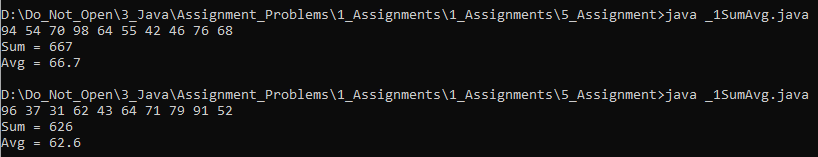
\includegraphics[width=0.8\textwidth]{1.png}
\end{center}

% 2

\section{Min and Max of array elements}
\textbf{Task:} Program to find min and max of array elements

\subsection{}
\begin{lstlisting}
class _2MinMax {
    public static void main(String[] args) {
        int[] arr = new int[10];
        for(int i=0; i<arr.length; i++)
            arr[i] = 1 + (int) (Math.random()*100);
    
        for(int i:arr)
            System.out.print(i + " ");
        System.out.println();
    
        int min = arr[0];
        int max = arr[0];
    
        for(int i=0; i<arr.length; i++) {
            if (arr[i] < min)
                min = arr[i];
            if (arr[i] > max)
                max = arr[i];
        }
        System.out.println("Max = "+max+" Min = "+min);
    }
}
\end{lstlisting}

\subsubsection{}
\begin{center}
    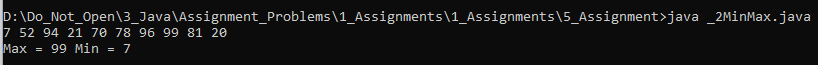
\includegraphics[width=0.8\textwidth]{2.png}
\end{center}

% 3

\section{Search Array Element}
\textbf{Task:} Program to search an element in array

\subsection{}
\begin{lstlisting}
import java.util.Scanner;
class _3Search {
    public static void main(String[] args) {
        Scanner sc = new Scanner(System.in);
        int[] arr = new int[100];
        for(int i=0; i<arr.length; i++)
            arr[i] = 1 + (int) (Math.random()*100);
        for(int i:arr)
            System.out.print(i + " ");
        System.out.println();
        System.out.print("Enter an element to search: ");
        int x = sc.nextInt();
        boolean flag = false;
    
        for(int i=0; i<arr.length; i++) {
            if (x == arr[i]){
                System.out.println("The Item "+x+" is found at "+i);
                flag = true;
                break;
            }
        }
    
        if (flag == false)
            System.out.println("The Item "+x+" is not found in the array");
    }
}
\end{lstlisting}

\subsubsection{}
\begin{center}
    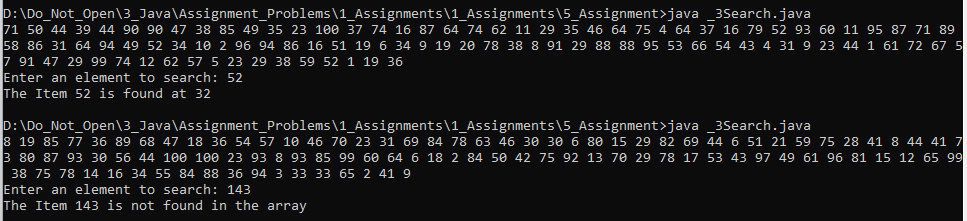
\includegraphics[width=0.8\textwidth]{3.png}
\end{center}

% 4

\section{Reverse Array Element}
\textbf{Task:} Program to reverse elements an array

\subsection{}
\begin{lstlisting}
class _4ReverseArray {
    public static void main(String[] args) {
        int[] arr = new int[10];
    
        for(int i=0; i<arr.length; i++)
            arr[i] = 1 + (int) (Math.random()*100);
    
        // original array
        for(int x:arr)
            System.out.print(x + " ");
        System.out.println();
    
        int[] reversedArr = new int[arr.length];
    
        for(int i=0; i<arr.length; i++)
            reversedArr[i] = arr[arr.length - 1 - i];
    
        // reversed array
        System.out.println("Reversed Array: ");
        for(int x:reversedArr)
            System.out.print(x+ " ");
    }
}
\end{lstlisting}

\subsubsection{}
\begin{center}
    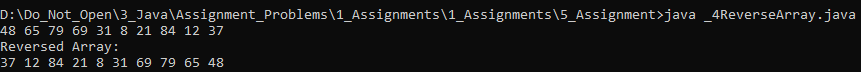
\includegraphics[width=0.8\textwidth]{4.png}
\end{center}

\section{Sort Array}
\textbf{Task:} Program to find a way to sort an array

% 5

\subsection{}
\begin{lstlisting}
import java.util.Arrays;
class _5SortArr {
    public static void main(String[] args) {
        int[] arr = new int[10];
    
        for(int i=0; i<arr.length; i++)
            arr[i] = 1 + (int) (Math.random()*100);
    
        // original array
        for(int x:arr)
            System.out.print(x + " ");
        System.out.println();
    
        Arrays.sort(arr);
    
        for(int i:arr)
            System.out.print(i + " ");
    }
}
\end{lstlisting}

\subsubsection{}
\begin{center}
    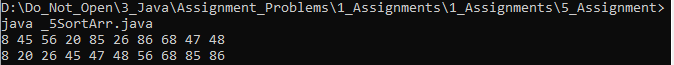
\includegraphics[width=0.8\textwidth]{5.png}
\end{center}

% 6

\section{Sum of squares of odd index values}
\textbf{Task:} Program to find sum of squares of odd index values

\subsection{}
\begin{lstlisting}
class _6SquaresOddValues {
    // Sum of squares of Odd Index Values
    public static void main(String[] args) {
        int[] arr = new int[10];
    
        for(int i=0; i<arr.length; i++)
            arr[i] = 1 + (int) (Math.random()*100);
    
        // original array
        for(int x:arr)
            System.out.print(x + " ");
        System.out.println();
    
        long sum = 0;
        for(int i=1; i<arr.length; i++){
            if (i % 2 !=0){
                sum += arr[i] * arr[i];
            }
        }
        System.out.println("Sum of squares of Odd Index Values: " + sum);
    }
}
\end{lstlisting}

\subsubsection{}
\begin{center}
    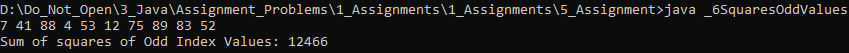
\includegraphics[width=0.8\textwidth]{6.png}
\end{center}

% 7

\section{First and Second Half of an Array}
\textbf{Task:} Program to find sum of first and second half of an array

\subsection{}
\begin{lstlisting}
class _7FirstSecondHalfSum {
    public static void main(String[] args) {
        int[] arr = new int[10];
    
        for(int i=0; i<arr.length; i++)
            arr[i] = 1 + (int) (Math.random()*100);
    
        // original array
        for(int x:arr)
            System.out.print(x + " ");
        System.out.println();
    
        int first = 0;
        int second = 0;
    
        for(int i=0; i<arr.length; i++){
            if (i <= (arr.length/2 - 1))
                first += arr[i];
            else 
                second += arr[i];
        }
    
        System.out.println("Sum of first half: " + first);
        System.out.println("Sum of second half: " + second);
    }
}
\end{lstlisting}

\subsubsection{}
\begin{center}
    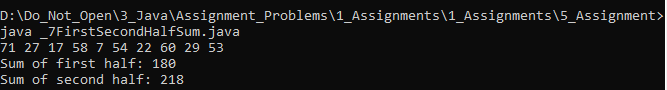
\includegraphics[width=0.8\textwidth]{7.png}
\end{center}

% 8

\section{Nth Largest/ Smallest}
\textbf{Task:} Program to find the nth largest / smallest element in the array

\subsection{}
\begin{lstlisting}
import java.util.Arrays;
import java.util.Scanner;
class _8Nth {
    public static void main(String[] args) {
        Scanner sc = new Scanner(System.in);
        int[] arr = new int[10];
    
        for(int i=0; i<arr.length; i++)
            arr[i] = 1 + (int) (Math.random()*100);
    
        // original array
        for(int x:arr)
            System.out.print(x + " ");
        System.out.println();
    
        Arrays.sort(arr);
    
        // sorted array
        for(int i:arr)
            System.out.print(i + " ");
    
        System.out.println();
    
        System.out.print("Enter to find the nth largest and smallest values: ");
        int n = sc.nextInt();
    
        if (n <= 0 || n > arr.length){
            System.out.println("Out of range");
            return;
        }
    
        int nthsmallest = arr[n-1];
        int nthlargest = arr[arr.length - n];
    
        System.out.println(n+"th smallest element is "+nthsmallest);
        System.out.println(n+"th largest element is "+nthlargest);
    }
}
\end{lstlisting}

\subsubsection{}
\begin{center}
    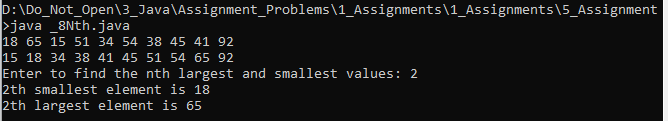
\includegraphics[width=0.8\textwidth]{8.png}
\end{center}

% 9

\section{Read and Print Array Elements}
\textbf{Task:} Program to read and print array elements

\subsection{}
\begin{lstlisting}
import java.util.Scanner;
class _9ReadPrintArray {
    public static void main(String[] args) {
        Scanner sc = new Scanner(System.in);
    
        // 1. Reading array elements from user input
        System.out.print("Enter the size of the array: ");
        int size = sc.nextInt();
    
        int[] userArr = new int[size];
    
        System.out.println("Enter " + size + " Integer Elements: ");
        for(int i=0; i<size; i++){
            System.out.print("Element " + (i + 1) + " : ");
            userArr[i] = sc.nextInt();
        }
        System.out.println();
        // 2. printing array elements
        for(int x:userArr)
            System.out.print(x + " ");
    }
}
\end{lstlisting}

\subsubsection{}
\begin{center}
    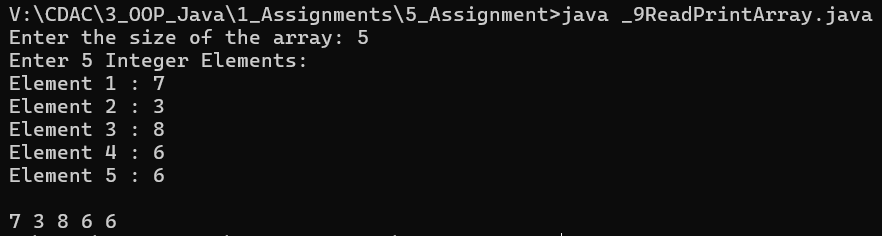
\includegraphics[width=0.8\textwidth]{9.png}
\end{center}

% 10

\section{Matrix Addition}
\textbf{Task:} Program to add two matrices

\subsection{}
\begin{lstlisting}
class _10MatrixAddition {
    public static void main(String[] args) {
        // Define two matrices
        int[][] matrixA = {
            {1, 2, 3},
            {4, 5, 6},
            {7, 8, 9}
        };
    
        int[][] matrixB = {
            {9, 8, 7},
            {6, 5, 4},
            {3, 2, 1}
        };
    
        // Get the dimensions of the matrices
        int rows = matrixA.length;
        int cols = matrixA[0].length;
    
        // Check if matrices can be added (same dimensions)
        if (rows != matrixB.length || cols != matrixB[0].length) {
            System.out.println("Matrices cannot be added. Dimensions mismatch.");
            return;
        }
    
        // Create a result matrix to store the sum
        int[][] sumMatrix = new int[rows][cols];
    
        // Perform matrix addition
        for (int i = 0; i < rows; i++) {
            for (int j = 0; j < cols; j++) {
                sumMatrix[i][j] = matrixA[i][j] + matrixB[i][j];
            }
        }
    
        for (int i = 0; i < sumMatrix.length; i++) {
            for (int j = 0; j < sumMatrix[0].length; j++) {
                System.out.print(sumMatrix[i][j] + " ");
            }
            System.out.println();
        }
    }
}
\end{lstlisting}

\subsubsection{}
\begin{center}
    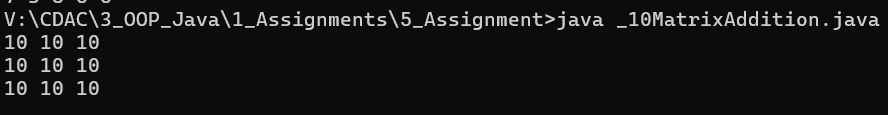
\includegraphics[width=0.8\textwidth]{10.png}
\end{center}

% 11 to 20

\section{Matrix Multiplication}
\textbf{Task:} Program to multiply two matrices

\subsection{}
\begin{lstlisting}
class _11MatrixMultiplication {
    public static void main(String[] args) {
        int[][] matrix1 = {{1, 2, 3}, {4, 5, 6}};
        int[][] matrix2 = {{7, 8}, {9, 10}, {11, 12}};
    
        int r1 = matrix1.length;
        int c1 = matrix1[0].length;
        int r2 = matrix2.length;
        int c2 = matrix2[0].length;
    
        // check
        if (c1 != r2) {
            System.out.println("Matrix Mutliplication not possible");
            return;
        }
    
        int[][] resultMatrix = new int[r1][c2];
    
        for(int i=0; i<r1; i++){
            for(int j=0; j<c2; j++){
                for(int k=0; k<c1; k++) {
                    resultMatrix[i][j] += matrix1[i][k] * matrix2[k][j];
                }
            }
        }
        System.out.println("Resultant Matrix: ");
    
        for (int i = 0; i < r1; i++) {
            for (int j = 0; j < c2; j++) {
                System.out.print(resultMatrix[i][j] + "\t");
            }
            System.out.println(); // New line after each row
        }
    }
}
\end{lstlisting}

\subsubsection{}
\begin{center}
    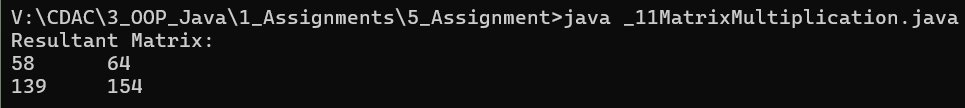
\includegraphics[width=0.8\textwidth]{11.png}
\end{center}

% 12

\section{Sum of diagonal elements}
\textbf{Task:} Program to find sum of diagonal elements

\subsection{}
\begin{lstlisting}
class _12MatrixDaignolSum {
    public static void main(String[] args) {
        int[][] myMatrix = {
            {1, 2, 3},
            {4, 5, 6},
            {7, 8, 9}
        };
    
        System.out.println("The matrix is:");
        for (int i = 0; i < myMatrix.length; i++) {
            for (int j = 0; j < myMatrix[i].length; j++) {
                System.out.print(myMatrix[i][j] + " ");
            }
            System.out.println();
        }
    
        int principalDiagonalSum = 0;
        int secondaryDiagonalSum = 0;
        int matrixSize = myMatrix.length; // Assuming a square matrix
    
        for (int i = 0; i < matrixSize; i++) {
            // Sum of principal diagonal elements
            principalDiagonalSum += myMatrix[i][i];
    
            // Sum of secondary diagonal elements
            secondaryDiagonalSum += myMatrix[i][matrixSize - 1 - i];
        }
    
        System.out.println("Sum of Principal Diagonal elements: " + principalDiagonalSum);
        System.out.println("Sum of Secondary Diagonal elements: " + secondaryDiagonalSum);
    }
    }

\end{lstlisting}

\subsubsection{}
\begin{center}
    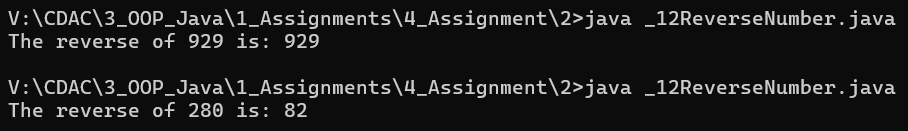
\includegraphics[width=0.8\textwidth]{12.png}
\end{center}



\end{document}
